\documentclass[aspectratio=169]{beamer}

\mode<presentation>
{
  \usetheme{default}
  \usecolortheme{default}
  \usefonttheme{default}
  \setbeamertemplate{navigation symbols}{}
  \setbeamertemplate{caption}[numbered]
  \setbeamertemplate{footline}[page number]
  \setbeamercolor{frametitle}{fg=white}
  \setbeamercolor{footline}{fg=black}
} 

\usepackage[english]{babel}
\usepackage[utf8x]{inputenc}
\usepackage{tikz}
\usepackage{listings}
\usepackage{courier}
\usepackage{array}
\usepackage{bold-extra}
\usepackage{minted}

\xdefinecolor{darkblue}{rgb}{0.1,0.1,0.7}
\xdefinecolor{darkgreen}{rgb}{0,0.5,0}
\xdefinecolor{darkgrey}{rgb}{0.35,0.35,0.35}
\xdefinecolor{darkorange}{rgb}{0.8,0.5,0}
\xdefinecolor{darkred}{rgb}{0.7,0,0}
\xdefinecolor{dianablue}{rgb}{0.18,0.24,0.31}
\definecolor{commentgreen}{rgb}{0,0.6,0}
\definecolor{stringmauve}{rgb}{0.58,0,0.82}

\lstset{ %
  backgroundcolor=\color{white},      % choose the background color
  basicstyle=\ttfamily\small,         % size of fonts used for the code
  breaklines=true,                    % automatic line breaking only at whitespace
  captionpos=b,                       % sets the caption-position to bottom
  commentstyle=\color{commentgreen},  % comment style
  escapeinside={\%*}{*)},             % if you want to add LaTeX within your code
  keywordstyle=\color{blue},          % keyword style
  stringstyle=\color{stringmauve},    % string literal style
  showstringspaces=false,
  showlines=true
}

\lstdefinelanguage{scala}{
  morekeywords={abstract,case,catch,class,def,%
    do,else,extends,false,final,finally,%
    for,if,implicit,import,match,mixin,%
    new,null,object,override,package,%
    private,protected,requires,return,sealed,%
    super,this,throw,trait,true,try,%
    type,val,var,while,with,yield},
  otherkeywords={=>,<-,<\%,<:,>:,\#,@},
  sensitive=true,
  morecomment=[l]{//},
  morecomment=[n]{/*}{*/},
  morestring=[b]",
  morestring=[b]',
  morestring=[b]"""
}

\title[2017-09-29-strangeloop]{Particle Physics, 10\,000 times faster}
\author{Jim Pivarski}
\institute{Princeton University -- DIANA}
\date{September 30, 2017}

\begin{document}

\logo{\pgfputat{\pgfxy(0.11, 7.4)}{\pgfbox[right,base]{\tikz{\filldraw[fill=dianablue, draw=none] (0 cm, 0 cm) rectangle (50 cm, 1 cm);}
\includegraphics[height=1 cm]{diana-hep-logo.png}}}}

\begin{frame}
  \titlepage
\end{frame}

% Uncomment these lines for an automatically generated outline.
%\begin{frame}{Outline}
%  \tableofcontents
%\end{frame}

%%%%%%%%%%%%%%%%%%%%%%%%%%%%%%%%%%%%%%%%%%%%%%%%%%%%%%%

\begin{frame}{Particle physics: the most industrial field of academia}
\vspace{0.15 cm}
\begin{columns}
\column{0.37\linewidth}
\begin{center}
\begin{minipage}{0.8\linewidth}

\textcolor{darkblue}{The goals are academic:} to explore strange new phenomena; to seek out new particles and new \mbox{interactions\ldots}

\vspace{0.5 cm}
\textcolor{darkblue}{The scale is industrial:} \mbox{billion} dollar hardware, planning on decadal time- scales, \mbox{millions} of lines of code\ldots

\vspace{0.5 cm}
\end{minipage}
\end{center}

\column{0.77\linewidth}
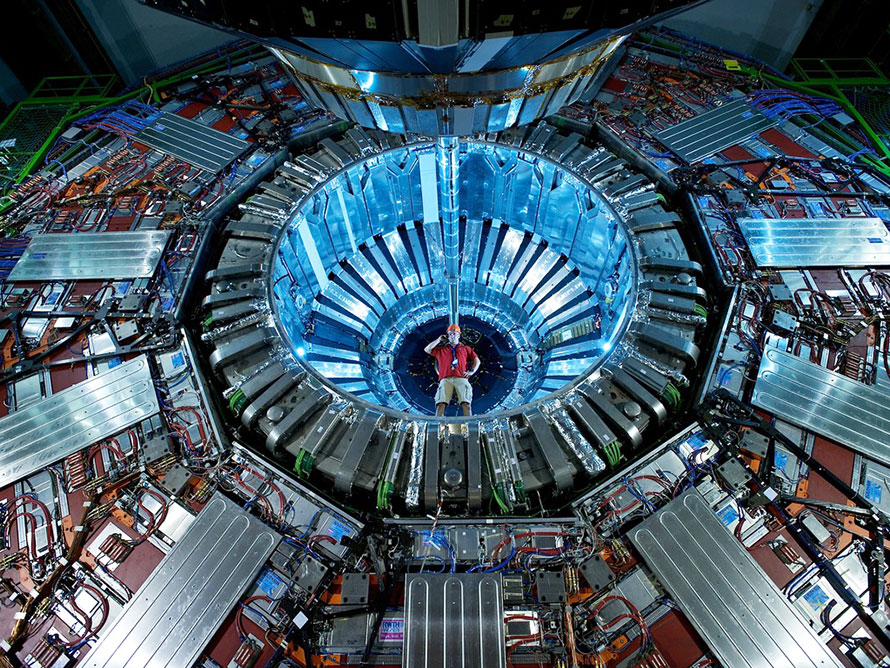
\includegraphics[width=\linewidth]{lhc-industrial-2.jpg}

\end{columns}
\end{frame}

\begin{frame}{It's big data\ldots\ \only<2->{but not {\it really} big}}
\vspace{0.35 cm}
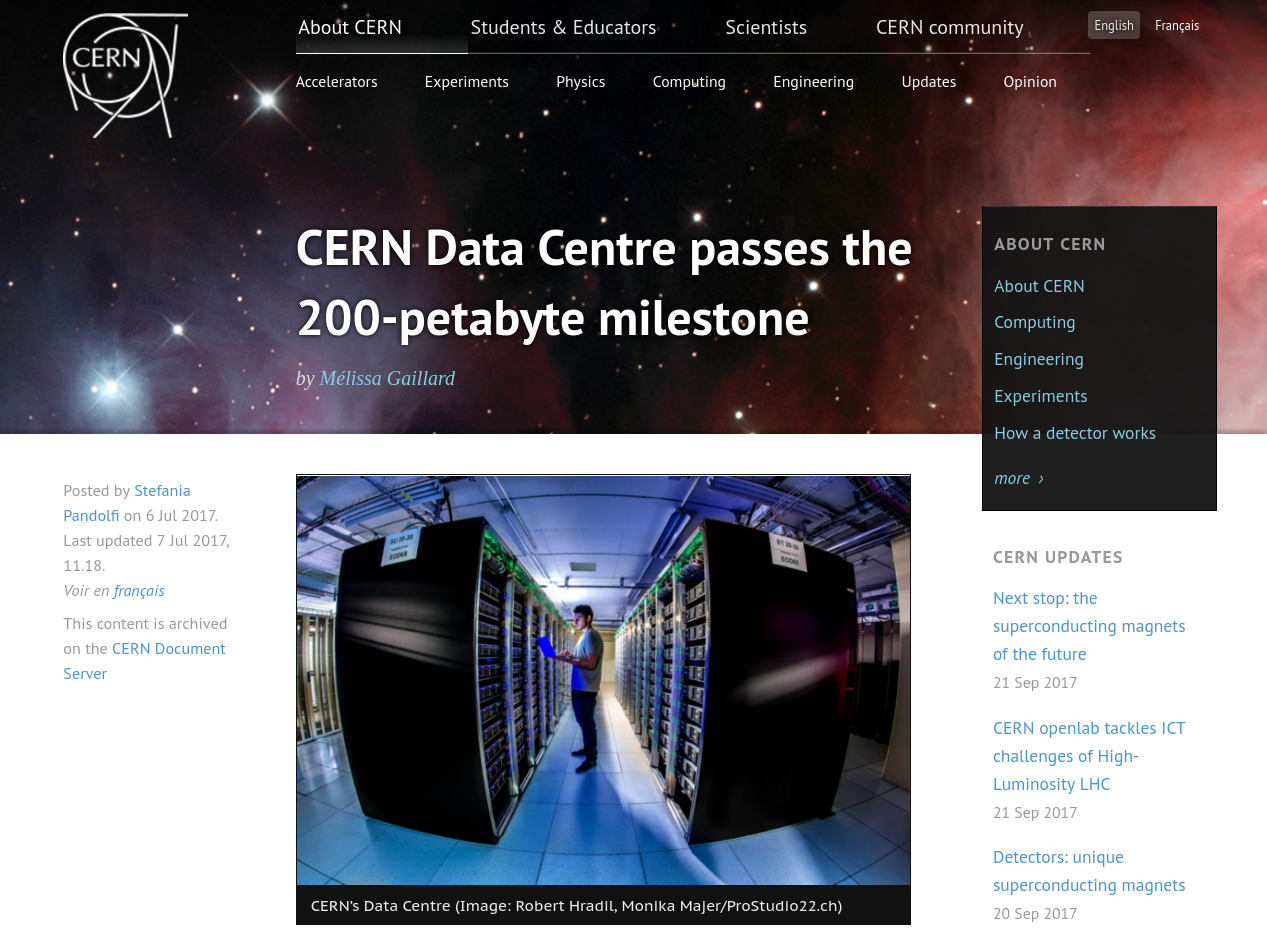
\includegraphics[width=0.73\linewidth]{cern-200pb.png}

\vspace{-4.8 cm}
\uncover<2->{\mbox{ } \hfill 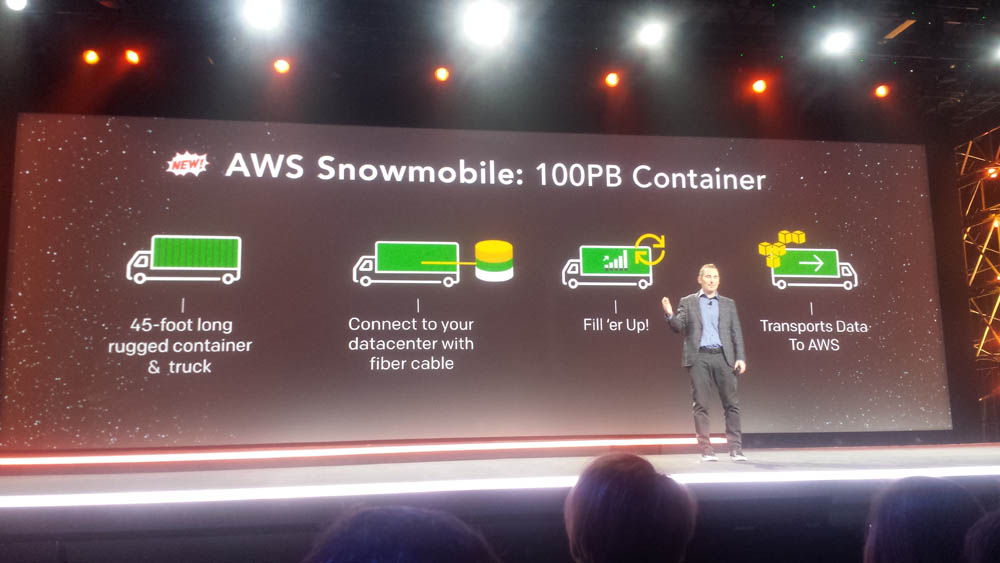
\includegraphics[width=0.7\linewidth]{aws-snowmobile.jpg}\hspace{-1 cm}}
\end{frame}

\begin{frame}{Our software developed before the big data ecosystem}
\vspace{0.25 cm}
It's my job to try to find ways to bridge the divide.

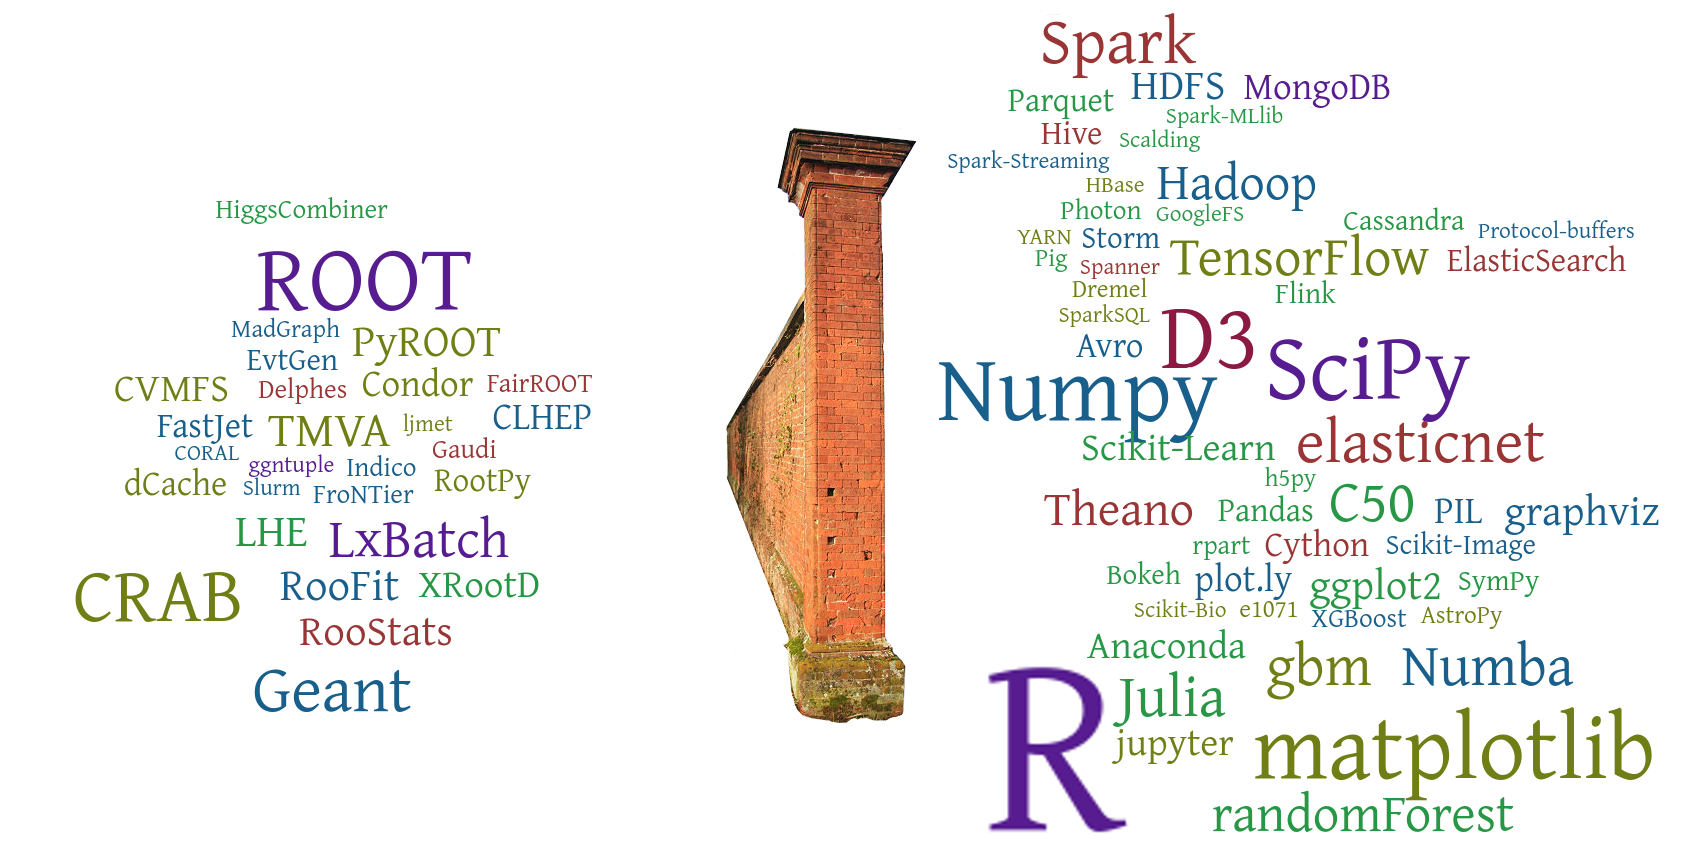
\includegraphics[width=\linewidth]{separation.png}
\end{frame}

\begin{frame}{}
\vspace{1 cm}
\large
\begin{center}
The obstacles are not just {\it accidental}--- artifacts of technology choice \\ (e.g.\ C++ in particle physics and Java in the Hadoop/Spark world).

\vspace{1 cm}
There are also {\it essential} qualities that current big data systems don't offer.

\vspace{1 cm}
\uncover<2->{This represents an {\it opportunity} on both sides: alien civilizations that evolved independenly can stand to learn a lot from each other.}
\end{center}
\end{frame}

\begin{frame}{So, what is unique about particle physics data?}

\begin{columns}
\column{1.15\linewidth}
\vspace{0.11 cm}
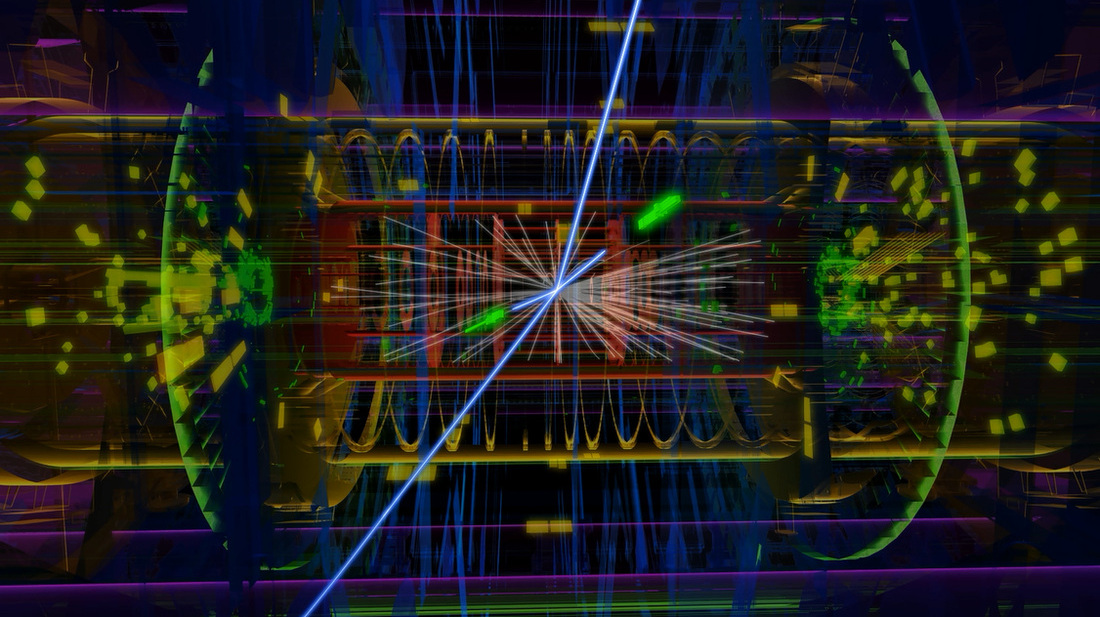
\includegraphics[width=\linewidth]{complex-atlas-collision-art.jpg}
\end{columns}

\vspace{-8.4 cm}
\uncover<2->{\textcolor{white}{\Huge\bf It's not the size.}}

\vspace{0.5 cm}
\uncover<3->{\textcolor{white}{\Huge\bf Arguably, it's the complexity.}}

\vspace{3.3 cm}
\uncover<4->{\textcolor{white}{\Huge\bf This picture represents one ``row'' in our data ``table.''}}

\vspace{8.4 cm}
\end{frame}

\begin{frame}{Particle physics data are not stored in databases}

\begin{itemize}\setlength{\itemsep}{0.5 cm}
\item We don't benefit from indexing, query planning, or high-level query languages.
\item<2-> Every data pull is a custom C++ program, accessing lists of files, taking months while the user chases down failures and stragglers.
\item<3-> But if our data {\it were} in a conventional (relational or NoSQL) database, the first thing we'd do is extract it and work with files again.
\end{itemize}
\begin{center}
\huge \uncover<3->{Why?}
\end{center}
\end{frame}

\begin{frame}
\vspace{0.5 cm}
\begin{columns}[t]
\column{0.5\linewidth}
\begin{center}
\Large Our data are deeply nested \\ and cross-linked

\vspace{-0.25 cm}
\rule{\linewidth}{0.8 pt}
\end{center}

\vspace{-0.25 cm}
\begin{itemize}\setlength{\itemsep}{0.5 cm}
\item<2-> Not a problem nowadays, as Drill, Parquet, and Arrow can explode nested structures into columns for fast, sparse access.

\vspace{0.2 cm}
\textcolor{gray}{(We've been doing it since the 90's.)}

\item<3-> Cross-links (pointers) could be supported by a graph database.

\vspace{0.2 cm}
\textcolor{gray}{(List indexes work well enough for our large number of small graphs.)}

\end{itemize}

\column{0.5\linewidth}
\begin{center}
\Large The operations we perform make intensive use of that structure

\vspace{-0.25 cm}
\rule{\linewidth}{0.8 pt}
\end{center}

\vspace{-0.25 cm}
\begin{itemize}
\item<4-> We frequently need to search sublists under constraints, optimize pairings, iterate over combinatorics\ldots

\item<5-> Even the simplest particle physics search criteria would require explodes, tags, and joins in SQL.

\vspace{0.2 cm}
\href{https://stackoverflow.com/q/38831961/1623645}{\textcolor{gray}{\scriptsize (https://stackoverflow.com/q/38831961/1623645)}}

\vspace{0.5 cm}
\begin{uncoverenv}<6->
To give a sense of the problem, I'll walk through a sample analysis.
\end{uncoverenv}
\end{itemize}
\end{columns}
\end{frame}






\begin{frame}{Publish with 5\,154 of your closest friends}
\vspace{0.5 cm}
(Author list of a recent paper)

\vspace{0.25 cm}
\includegraphics[width=\linewidth]{authors.pdf}
\end{frame}

\end{document}
